% !TeX spellcheck = pt_BR
\documentclass[tese_patricia]{subfiles}
\begin{document}
	
	\begin{comment}
		\nomenclature[G,01]{$\Omega_{IFE}$}{Domínio computacional de problemas de Interação Fluido Estrutura;}
		\nomenclature[G,02]{$._{F}, ._{E}, ._{M}$}{Subíndices que designam fluido, estrutura e malha respectivamente;}
		\nomenclature[G,03]{$\Gamma_{IFE}$}{Contorno que define a interface fluido-estrutura;}
		\nomenclature[G,04]{$\mathbf{n}$}{Vetor normal ao contorno $\Gamma_{IFE}$;}
		\nomenclature[G,05]{$._{\tilde{t}}$}{Subíndice que designa tempo de referência$;}
		\nomenclature[G,06]{$\testfunction$}{Função peso respectiva ao deslocamento da malha;}
		\nomenclature[G,07]{$\mathbf{z}$}{Vetor de deslocamentos da malha;}
		\nomenclature[G,8]{$E_m$}{Módulo de elasticidade fictício da malha;}
		\nomenclature[G,9]{$JM$}{Jacobiano da malha;}
		\nomenclature[G,10]{$(JM)_{0}$}{Parâmetro livre;}
		\nomenclature[G,11]{$\chi$}{Parâmetro que determina a ordem pelo qual os elementos menores serão enrijecidos mais do que os maiores;}
		\nomenclature[G,12]{$\mathbf{N}_{i}$}{Equação que descreve o comportamento do problema de IFE com i = 1,3 (1- fluido, 2-estrutura e 3-malha);}
		\nomenclature[G,13]{$\mathbf{d}_{i}$}{Vetores com as variáveis nodais do problema de IFE com i = 1,3 (1- fluido, 2-estrutura e 3-malha);}
		\nomenclature[G,14]{$\mathbf{A_{ij}}$}{$\mathbf{A_{ij}} = \frac{\partial\mathbf{N}_{i}}{\partial\mathbf{d}_{j}}$;}
		\nomenclature[G,15]{$\mathbf{x}_{i}$}{Incremento as soluções  $\mathbf{d}_{i}$;}
		\nomenclature[G,16]{$\mathbf{b}_{i}$}{$\mathbf{b}_{i} = -\mathbf{N}_{i}$}
		\nomenclature[G,17]{$\mathbf{t^{E}}$}{Forças de superfície no contorno $\Gamma_{IFE}$ aplicadas a estrutura;}
		\nomenclature[G,18]{$h$}{Espessura da placa;}
		\nomenclature[G,19]{$f_{f}$}{Frequência de desprendimento de vórtices do fluido;}
		\nomenclature[G,19]{$f_{i}$}{i-ésima frequência natural da estrutura;}
		
		
		NÃO COLOQUEI TENSOR DE DEFORMAÇÕES E NEM DE TENSÕES, JÁ DEVEM ESTAR EM OUTRO PONTO;
		NÃO COLOQUEI AS VARIÁVEIS COM ÍNDICES H, E BARRA;
		NÃO COLOQUEI COORDENADAS PARAMÉTRICAS MESMO COM ÍNDICES E, F.
		NÃO COLOQUEI MEDIDA DE CONVERGÊNCIA EPSLON já deve estar em outro local
		
	\end{comment}

% ---------------------------------------------------------- 
% Métodos de malhas sobrepostas
% ----------------------------------------------------------
\chapter[Acoplamento Fluido-Estrutura]{Interação Fluido-Estrutura} \label{capitulo:Cap7}
% ----------------------------------------------------------


Ao longo deste trabalho, conforme apresentado nos capítulos anteriores, foi desenvolvido um código computacional para análise de fluidos incompressíveis que permite a decomposição do domínio para capturar efeitos localizados por meio da técnica Arlequin estabilizada. Além disso, para esta pesquisa, foi disponibilizado por um pesquisador do grupo de pesquisas em Mecânica Computacional do Departamento de Engenharia de Estruturas da Escola de Engenharia de São Carlos, no qual a presente aluna está inserida, um código computacional para a análise não linear de estruturas pelo método dos elementos finitos posicional. Com base nesses desenvolvimentos, optou-se por um esquema de acoplamento particionado forte entre fluido e estrutura. Essa abordagem foi escolhida por proporcionar um total desacoplamento entre os \textit{solvers} de fluido e de estrutura, o que facilita a solução dos problemas que aqui serão propostos.

Nesse contexto, para o acoplamento, utiliza-se a técnica de malhas adaptadas para a malha local do fluido em contato com a estrutura, aplicando-se uma descrição ALE. Vale ressaltar que, embora a malha local possa se mover, a malha global permanece fixa com descrição Euleriana, fazendo com que o método de acoplamento possa ser classificado como uma técnica híbrida.
 
No texto a seguir descrevem-se as condições de acoplamento necessárias a solução de um problema IFE, a técnica de movimentação de malha utilizada nesse estudo, e a metodologia de transferência de condições de contorno (Dirichlet-Neumann) em uma interface de fluido e sólido com malha não coincidente. Discorre-se na continuação sobre os detalhes a cerca do esquema de acoplamento particionado forte adotado. Por fim, o algoritmo de implementação computacional será apresentado, e exemplos de validação serão exibidos na sequência.

\section{Condições de acoplamento}

O domínio computacional para a análise de problemas de interação fluido-estrutura (Fig. \ref{fig:dominios}), denominado de $\Omega_{IFE}$, é composto pela união entre os domínios da estrutura $\Omega_E$ e do fluido $\Omega_F$, ou seja, $\Omega_{IFE} = \Omega_F \cup \Omega_E$, com $\Gamma_{IFE}$ representando o contorno que define a interface fluido-estrutura.

\begin{figure}[htb!]
	\centering 
	%\vspace{-1em} % Diminui o espaço antes da figura
	\includegraphics[scale=1.0,trim=0cm 0cm 0cm 0.0cm, clip=true]{Imagens/Cap7/dominio.pdf}	
	\caption{Domínios Computacional para análise de problemas de IFE.}
	\label{fig:dominios}
	%\vspace{-1em} % Diminui o espaço antes da figura
\end{figure}

O domínio computacional não se sobrepõe, por isso, é necessário que em $\Gamma_{IFE}$ existam condições físicas adicionais para se realizar o acoplamento. \citeonline{richter2017fluid} cita que o acoplamento é realizado através de 3 diferentes princípios no contorno $\Gamma_{IFE}$ : condição cinemática, condição dinâmica e condição geométrica.

A condição cinemática refere-se ao fato de que a velocidade do fluido e do sólido na interface devem ser iguais. A condição dinâmica, refere-se à existência de continuidade do vetor tensão de Cauchy na direção normal ao contorno $\Gamma_{IFE}$.

Em esquemas de acoplamento monolítico, as condições cinemática e dinâmica são atendidas de maneira implícita, visto que os meios são tratados no mesmo contexto matemático. Para esquemas particionadas, como o desse estudo, essas condições são atendidas através da transferência de condições de contorno apropriadas entre os meios.

Para a condição cinemática têm-se:

\begin{align}
	\velocityh = \solidVel^h \ \textrm{no contorno} \ \Gamma_{IFE},
\end{align}

\noindent atendida através da aplicação dos valores de $\solidVel^h$ nos nós (ou pontos de controle) que compõe a malha do fluido na interface entre os meios.

A condição dinâmica, preescreve o balanço da tensão normal no contorno, ao que diz respeito à ação e reação, conforme a equação abaixo:

\begin{align}
	\mathbf{\sigma}_{E}\mathbf{n}_{E} + \mathbf{\sigma}_{F}\mathbf{n}_{F} = 0 \ \textrm{no contorno} \ \Gamma_{IFE},
\end{align}

\noindent na qual, $\mathbf{\sigma}_{E}$ representa as tensões de Cauchy da estrutura, $\mathbf{\sigma}_{F}$ as tensões de Cauchy no fluido, e $\mathbf{n}_E$ e $\mathbf{n}_F$ representam o vetor normal no contorno $\Gamma_{IFE}$ respectivamente apontando para o fluido e para a estrutura. Essa condição é atendida através da aplicação de $\mathbf{\sigma}_{F}\mathbf{n}_{F}$ aos nós da malha da estrutura na interface entre os meios.

Já a condição geométrica está relacionada ao fato que os domínios computacionais $\Omega_E$ da estrutura e $\Omega_F$ do fluido devem sempre coincidir em $\Gamma_{IFE}$, ou seja, não devem existir superposições ou frestas nessa interface. No contexto desse estudo essa condição é atendida através de uma movimentação adequada da malha local (Método Arlequin), que se deforma para acomodar a mudança de configuração da estrutura. A técnica de movimentação de malha adotada será apresentada na Subseção \ref{subsec:MovMalha}.

\subsection{Movimentação da Malha} \label{subsec:MovMalha}

Para a satisfação da condição geométrica nos problemas de IFE desse trabalho, uma técnica adequada de movimentação de malha deve ser aplicada. É necessário que o método de movimentação de malha seja robusto o suficiente para que garanta ao longo de toda a análise dos problemas uma discretização de qualidade.

Dentre as técnicas desenvolvidas até o momento, destacam-se aquelas que impõem os deslocamentos da estrutura na malha do fluido ao longo do contorno $\Gamma_{IFE}$, determinando o campo de deslocamentos na malha do fluido por meio da resolução de um problema de valor de contorno (PVC). Neste trabalho, será adotada essa abordagem, formulando o problema com base na equivalência entre a movimentação da malha à um problema de mecânica dos sólidos, e aplicando-se a técnica de movimentação de malhas introduzida em \citeonline{TezduyarBSJ:1992f} e \citeonline{TezduyarABJ:1993} conhecida como MJBS (\textit{Mesh-Jacobian Based Stiffening}).

Nesse método, o movimento da malha é determinado usando um problema da elasticidade de Dirichlet fictício, descrito como:

\begin{align}
	\int_{\domaintt} \straintensor \left(\testfunction\right) : \stresstensor \left(\displacementmesh - \displacementmesh_{\tilde{t}}\right) d\Omega = 0,
	\label{eq:elasticityequation}
\end{align}


\noindent na qual $\testfunction$ é a função peso respectiva ao deslocamento da malha  $\displacementmesh$, medido a partir de uma configuração de referência até a configuração atual $\currentcoordinates$ e 
$\displacementmesh_{\tilde{t}}$ representa o deslocamento da configuração de referência até a malha no tempo ${\tilde{t}}$, ou $\currentcoordinates_{\tilde{t}}$. 
A escolha para ${\tilde{t}}$ é geralmente ${\tilde{t}} = {t_{n}}$ quando se calcula a configuração da malha no tempo ${t_{n+1}}$ (ver \citeonline{Tononetal:2021} para maiores detalhes). 

O tensor de tensões é calculado através da seguinte relação:

\begin{align}
	\stresstensor(\disp)
	&=
	\frac{E_m}{1+\poisonsRatio_m}
	\left(
	\frac{\poisonsRatio_m}{(1 - 2 \poisonsRatio_m)}
	\trace\left(\straintensor(\disp)\right)\unittensor
	+
	\straintensor(\disp)
	\right)
\end{align}

\noindent com $E_m$ e $\poisonsRatio_m$ o módulo de Elasticidade e o coeficiente de Poisson fictícios da malha respectivamente. Os valores usados por definição nesse trabalho são $E_m=1,0$ e $\poisonsRatio_m = 0,3$.

Nos problemas de IFE, demanda-se maior controle da resolução da malha próxima a interface dos meios fluidos e sólidos, para representar os efeitos de camada limite, e como consequência, a obtenção de soluções mais acuradas nessas regiões críticas. Para fazer com que na deformação da malha se leve em conta o tamanho dos elementos, enrijecendo os menores mais do que os maiores, no método MJBS a equação da elasticidade fica descrita ao final como:

\begin{align}
	\int_{\domaintt} \straintensor \left(\testfunction\right) : \stresstensor \left(\displacementmesh- \displacementmesh_{\tilde{t}}\right) \left(\frac{J_M}{\left({J_M}\right)_0}\right)^{-\chi} d\Omega = 0, 
	\label{eq:MJBS}
\end{align}

\noindent onde $J_M$ é o Jacobiano da malha, $(J_M)_0$ é um parâmetro livre e $\chi$ determina a ordem pela qual os elementos menores serão enrijecidos mais do que os maiores.  $\chi$ é adotado correntemente como 1. E o Jacobiano da malha calculado da forma que se segue:

\begin{align}
	J_M = det\left(\frac{\partial\currentcoordinates_{\tilde{t}}}{\partial\adimensionalcoordinates}\right), 
	\label{eq:3}
\end{align}

\noindent onde $\adimensionalcoordinates$ são as coordenadas paramétricas do elemento.

\section{Discretizações não coincidentes entre os meios}

Na maioria dos casos a discretização das malhas do fluido e da estrutura são não-coincidentes no contorno $\Gamma_{IFE}$ e podem inclusive ter aproximações matemáticas distintas. Dessa forma, uma metodologia que possibilita a aplicação de condições de contorno em caso de discretizações com nós não coincidentes, é imprescindível. 

O procedimento adotado nesse trabalho pode ser entendido a partir da Fig. \ref{fig:contornoIFE}. Nele, durante o pré-processamento do código computacional, cada nó do contorno da estrutura $\mathbf{x_E}$ é projetado sobre o contorno do fluido, e busca-se a coordenada paramétrica relativa a este ponto definida como $\boldsymbol{\xi_{F}}(\mathbf{x_E})$. Da mesma forma, cada nó do contorno do fluido $\mathbf{x_F}$ é projetado sobre o contorno da estrutura, e encontra-se uma coordenada paramétrica equivalente $\boldsymbol{\xi_{E}}(\mathbf{x_F})$. 


\begin{figure}[htb!]
	\centering 
	\includegraphics[scale=0.9,trim=0cm 0cm 0cm 0cm, clip=true]{Imagens/Cap7/contornoIFE.pdf}	
	\caption{Discretizações não-coincidentes no contorno IFE}
	\label{fig:contornoIFE}
\end{figure}

Dessa forma, as informações que serão transmitidas ao fluido pela estrutura são interpoladas na malha da estrutura em cada uma das coordenadas paramétricas que possuem um nó equivalente na malha de fluido, e após isso aplicadas a este nó. O equivalente ocorre quando os dados são provenientes do fluido e serão transmitidos a estrutura.


\section{Acoplamento Particionado Forte - Bloco-Iterativo}

Os problemas de IFE são caracterizados pela interdependência entre o fluido e a estrutura, visto que o comportamento do escoamento depende do formato e do movimento da estrutura, enquanto que o movimento da estrutura e sua deformação dependem das forças do fluido que atuam sobre ela. Matematicamente pode-se dizer que os problemas de IFE são conjuntos de equações e condições de contorno associadas ao fluido e a estrutura que devem ser satisfeitas simultaneamente.

As equações completas discretizadas da formulação IFE conduzem a um sistema de equações não-lineares que devem ser resolvidas a cada passo de tempo e podem ser representadas da seguinte maneira \cite{BazilevsTT:2013}:

\begin{align}
	\mathbf{N}_{1}\left(\mathbf{d}_{1},\mathbf{d}_{2},\mathbf{d}_{3}\right) = 0, \label{eq:N1}\\ 
	\mathbf{N}_{2}\left(\mathbf{d}_{1},\mathbf{d}_{2},\mathbf{d}_{3}\right) = 0,\label{eq:N2}\\
	\mathbf{N}_{3}\left(\mathbf{d}_{1},\mathbf{d}_{2},\mathbf{d}_{3}\right) = 0 \label{eq:N3},
\end{align}

\noindent em que $\mathbf{{N}_{1}}$, $\mathbf{{N}_{2}}$ e $\mathbf{{N}_{3}}$ representam as equações que descrevem o fluido, a estrutura e a malha respectivamente, e, $\mathbf{{d}_{1}}$, $\mathbf{{d}_{2}}$, $\mathbf{{d}_{3}}$ são vetores com as variáveis nodais de cada meio. 
A resolução dessas equações através do método de Newton-Raphson conduz ao seguinte sistema linear de equações:

\begin{align}
	\begin{bmatrix}
		\mathbf{A_{11}} & \mathbf{A_{12}} & \mathbf{A_{13}} \\
		\mathbf{A_{21}} & \mathbf{A_{22}} & \mathbf{A_{23}} \\
		\mathbf{A_{31}} & \mathbf{A_{32}} & \mathbf{A_{33}} 
	\end{bmatrix}
	\begin{bmatrix}
		\mathbf{x_{1}} \\
		\mathbf{x_{2}} \\
		\mathbf{x_{3}}
	\end{bmatrix}
	&=
	\begin{bmatrix}
		\mathbf{b_{1}} \\
		\mathbf{b_{2}} \\
		\mathbf{b_{3}}
	\end{bmatrix}.
	\label{eq:SistLinear}
\end{align}	

\noindent sendo $\mathbf{b_{1}} = - \mathbf{N}_{1}$, $\mathbf{b_{2}} = - \mathbf{N}_{2}$, $\mathbf{b_{3}} = - \mathbf{N}_{3}$. $\mathbf{x_{1}}$, $\mathbf{x_{2}}$ e $\mathbf{x_{3}}$ são os incrementos às soluções $\mathbf{d}_{1}$, $\mathbf{d}_{2}$ e $\mathbf{d}_{3}$ respectivamente e $\mathbf{A_{ij}} = \frac{\partial\mathbf{N}_{i}}{\partial\mathbf{d}_{j}}$. 

 \citeonline{BazilevsTT:2013} apresentam uma classificação da metodologia de acoplamento segundo a forma de resolver essas equações não-lineares. As categorias definidas pelos autores são: técnica direta, técnica bloco-iterativa e técnica quase-direta. 

A técnica direta seria equivalente aos esquemas de solução monolíticos citados ao longo do texto, e consiste na resolução a cada iteração de Newton-Raphson do sistema apresentado na Eq. \refeq{eq:SistLinear}. Essa técnica apresenta boa convergência, entretanto, devido aos grandes sistemas lineares gerados, ocorre um aumento do custo computacional.

Nesse contexto, e buscando proporcionar um total desacoplamento entre os \textit{solvers} de fluido e de estrutura, adotou-se o um esquema de acoplamento do tipo particionado forte. Dentro da classificação dos autores \citeonline{BazilevsTT:2013} seria equivalente a técnica de acoplamento do tipo bloco iterativo.

Quando se utiliza um acoplamento do tipo bloco iterativo, os sistemas do fluido, da estrutura e da malha são tratados em blocos separados, e para cada iteração dentro de um passo de tempo, se resolve sequencialmente o seguinte conjunto de equações:


\begin{align}
	\left .\frac{\partial\mathbf{N}_{1}}{\partial\mathbf{d}_{1}}\right|_{\left(\mathbf{d}_{1}^{i},\mathbf{d}_{2}^{i},\mathbf{d}_{3}^{i}\right)} \Delta\mathbf{d}_{1}^{i} = - \mathbf{N}_{1}\left(\mathbf{d}_{1}^{i},\mathbf{d}_{2}^{i},\mathbf{d}_{3}^{i}\right)  \label{eq:Fluido} \\
	\mathbf{d}_{1}^{i+1} =  \mathbf{d}_{1}^{i} + \Delta\mathbf{d}_{1}^{i} \label{eq:upFluido}	\\
	\left.\frac{\partial\mathbf{N}_{2}}{\partial\mathbf{d}_{2}}\right|_{\left(\mathbf{d}_{1}^{i+1},\mathbf{d}_{2}^{i},\mathbf{d}_{3}^{i}\right)} \Delta\mathbf{d}_{2}^{i} = - \mathbf{N}_{2}\left(\mathbf{d}_{1}^{i+1},\mathbf{d}_{2}^{i},\mathbf{d}_{3}^{i}\right) \label{eq:Estrutura}\\
	\mathbf{d}_{2}^{i+1} =  \mathbf{d}_{2}^{i} + \Delta\mathbf{d}_{2}^{i} \label{eq:upEstrutura}\\
	\left.\frac{\partial\mathbf{N}_{3}}{\partial\mathbf{d}_{3}}\right|_{\left(\mathbf{d}_{1}^{i+1},\mathbf{d}_{2}^{i+1},\mathbf{d}_{3}^{i}\right)} \Delta\mathbf{d}_{3}^{i} = - \mathbf{N}_{3}\left(\mathbf{d}_{1}^{i+1},\mathbf{d}_{2}^{i+1},\mathbf{d}_{3}^{i}\right) \label{eq:Malha}\\
	\mathbf{d}_{3}^{i+1} =  \mathbf{d}_{3}^{i} + \Delta\mathbf{d}_{3}^{i}  \label{eq:upMalha}
\end{align}

Nota-se que o ocorre é apenas uma modificação da matriz tangente com relação ao método direto. Este fato, faz com que a resposta não seja alterada, entretanto, a convergência do problema pode ser afetada. 

Em certos problemas envolvendo estruturas leves, a resposta estrutural pode tornar-se extremamente sensível a pequenas variações nas forças provenientes do fluido. Esse fenômeno pode levar à divergência da técnica de bloco iterativo. Para contornar essa dificuldade, adotou-se a estratégia proposta por \citeonline{Tezduyar:2003d}, chamada de \textit{Augmented A22} na qual a matriz de massa em $\mathbf{A_{22}}$ é aumentada por um fator dependente do tipo de problema em análise. Essa modificação ocorre sem alterar $\mathbf{b_{1}}$, $\mathbf{b_{2}}$ e $\mathbf{b_{3}}$, ou seja, sem modificar as equações não lineares. Dessa forma, quando a solução pelo método de bloco iterativo converge, a massa estrutural real do problema permanece inalterada.

\subsection{Implementação Computacional} 


O Algoritmo que descreve a implementação computacional do problema de IFE de acordo com a técnica de acoplamento forte do tipo bloco-iterativo é apresentada no Alg. \ref{alg:IFE}.

\begin{algorithm}
	\caption{Algoritmo para solução de problemas IFE}
	\label{alg:IFE}
	\begin{algorithmic}[1]
		\State Busca por coordenadas paramétricas correspondentes aos nós da malha do fluido na malha da estrutura;
		\State Busca por coordenadas paramétricas correspondentes aos nós da malha da estrutura na malha do fluido;
		\For {o passo de tempo $t=0$ até $t=\timeInterval$} 
		\State Atualiza as variáveis do fluido, estrutura e malha no passo de tempo $t = t-1$;
		\For {número de iterações de Newton Raphson $it=0$ até $it=N_{it}$}
		\State \textbf{Fluido}
		\State Realiza os passos das linhas 1., 2., 3. e 4. do Algoritmo \ref{alg:fluid_temporalIntegrationARLQ};
		\State Resolve o problema do fluido (Eq. \eqref{eq:Fluido});
		\State Atualiza as variáveis do fluido na iteração $it$ através da eq. \ref{eq:upFluido};
		\State Calcula medida de convergência $\epsilon_F$;
		\State Atualiza as forças de superfície no contorno  $\Gamma_{IFE}$ ($\boldsymbol{t^{E}} = -\boldsymbol{\sigma_{F}} \cdot \boldsymbol{n_{F}}$) ;
		\State \textbf{Estrutura}
		\State Resolve o problema da estrutura (Eq. \eqref{eq:Estrutura});
		\State Atualiza as variáveis da estrutura na iteração $it$ através da eq. \eqref{eq:upEstrutura};
		\State Calcula medida de convergênci0cma $\epsilon_E$;
		\State Atualiza velocidade e acelerações no fluido no contorno  $\Gamma_{IFE}$;
		\State Atualiza posição da interface da malha no contorno  $\Gamma_{IFE}$;
		\State \textbf{Malha}
		\State Resolve o problema de malha Eq. \eqref{eq:Malha};
		\State Atualiza as variáveis da malha na iteração $it$ através da eq. \eqref{eq:upMalha};
		\State Calcula medida de convergência $\epsilon_M$;
		\If    {$\epsilon_F$, $\epsilon_E$ e $\epsilon_M$ < $tol$ } 
		\State Sair do loop;
		\EndIf
		\EndFor
		\EndFor
	\end{algorithmic}
\end{algorithm}

No algoritmo apresentado $\boldsymbol{t^{E}}$ representa as forças de superfície no contorno $\Gamma_{IFE}$ aplicadas à estrutura, e as medidas de convergência $\epsilon_F$, $\epsilon_E$ e $\epsilon_M$ são normas vetoriais $L_2$ aplicadas sobre o resíduo das respectivas equações diferenciais.


\section{Exemplos}

Para a validação da metodologia de análise de problemas de IFE, apresentada nesse capítulo, alguns exemplos serão estudados e analisados.

Os dois primeiros exemplos dizem respeito a uma cavidade com um fundo flexível composto por uma chapa, com velocidade oscilatória aplicada em seu topo. Esses exemplos são uma extensão do típico problema da DFC de uma cavidade quadrada (apresentado, por exemplo, na Seção \ref{subsec:CavQua3d} em sua versão 3D) e serão apresentados em uma versão bidimensional e tridimensional.

O seguinte exemplo consiste em um painel flexível engastado a um bloco prismático rígido. Esse problema é comumente utilizado na validação de códigos de Interação Fluido-Estrutura (IFE), pois envolve fenômenos complexos. À medida que ocorre o desprendimento de vórtices devido ao escoamento ao redor do prisma, perturbações são geradas no fluxo, excitando a estrutura, que então sofre grandes deslocamentos.

\subsection{Cavidade com fundo flexível - 2D}

O problema da cavidade com fundo flexível trata-se de uma extensão do típico problema da DFC de uma cavidade quadrada com velocidade prescrita em sua parede superior. Sua simulação computacional já foi realizada por diversos autores, como por exemplo, \citeonline{GerbeauV:2003} e \citeonline{Yokomizo:2024}, e  por isso, será utilizada no processo de validação da metodologia nesta tese apresentada.

A cavidade com fundo flexível (geometria apresentada na Fig. \ref{fig:cavidadeFF2d:Geo}) consiste em uma cavidade composta por paredes laterais rígidas e um fundo flexível composto por uma placa fina de 0,002. No seu topo uma velocidade oscilatória horizontal $u_x(t)=1-cos(0,4 \pi t)$ é aplicada, sendo as demais velocidades ($u_y$ e $u_z$) nessa parede nulas. Condições de contorno de não deslizamento são aplicadas as paredes laterais. Esse modelo de cavidade apresenta duas aberturas de 0,1 no topo de suas laterais com condições homogêneas de Neumann. Como o problema apresenta comportamento bidimensional o mesmo será analisado utilizando-se uma discretização 3D com uma espessura de 0,1 de profundidade. Adotou-se condição de simetria para o fluido na direção $y$.  Na Fig. \ref{fig:cavidadeFF2d:Geo} são apresentadas também as propriedades físicas do fluido e da estrutura necessárias a análise.

\begin{figure}[htb!]
	\centering 
	\includegraphics[scale=1.3,trim=0cm 0cm 0cm 0cm, clip=true]{Imagens/Cap7/cav2d.pdf}	
	\caption{Cavidade fundo flexível 2D: geometria}
	\label{fig:cavidadeFF2d:Geo}
\end{figure}

A placa fina possui condições de deslocamentos nulos em suas laterais esquerda e direita, e, na direção perpendicular ao plano da cavidade o vetor generalizado e os deslocamentos, nesta direção, são prescritos como zero em $y=0,0$ e $y=0,1$.

No que diz respeito a integração temporal utilizou-se $\timeStep = 0,1$, e $\specRadius = 0,0$. A escolha por uma integração temporal com máxima dissipação se deu por conta do trabalho de \citeonline{Forsteretal:2007} que reporta que a regra trapezoidal de integração leva a resultados instáveis para esse problema.

Foram utilizadas nas análises três diferentes discretizações para o modelo Arlequin, sendo as malhas globais em elementos isogeométricos quadráticos (IGA) e as malhas locais, mais refinadas, em elementos finitos (MEF) tetraédricos quadráticos. Além disso, os resultados foram comparados com uma discretização somente em elementos finitos tetraédricos quadráticos, chamada de monomodelo. A quantidade de nós, ou pontos de controle (PC), e de elementos para cada uma dessas discretizações é apresentada na Tab. \ref{tab:CF2DD}, assim como detalhes da discretização da placa, na qual foram utilizados elementos triangulares quadráticos. Na tabela ML e MG são abreviações para malha local e malha global respectivamente.
	
	\begin{center}
		\begin{table}[h!]
			\caption{Discretizações}
			\centering
			\begin{tabular}{|c | c | c| c| c|} 
				\hline
				\ &  Nós/PC ML & Elementos ML & Nós/PC MG & Elementos MG  \\ 
				\hline
				Arlequin - Malha 0 & 777 & 370 & 504 & 100 \\ 
				\hline
				Arlequin - Malha 1 & 1625 & 778 & 1584 & 400\\
				\hline
				Arlequin - Malha 2 & 6156 & 3040 & 5544 & 1600\\
				\hline
				Monomodelo & - & - & 11789 & 5750\\
				\hline
				Estrutura - Malha 0 & - & - &  103 & 40\\
				\hline
				Estrutura - Malha 1 & - & - &  203 & 80\\
				\hline
				Estrutura - Malha 2 & - & - &  883 & 400\\
				\hline
			\end{tabular}
			\label{tab:CF2DD}
		\end{table}
	\end{center}


A malha isogeométrica utilizada foi composta por 2 \textit{patches} (observar Fig. \ref{fig:cavidadeFF2d:Malhas}). Essa discretização usando 2 \textit{patches} foi necessária para gerar pontos de controle interpolatórios posicionados na linha que separa as paredes laterais das aberturas, possibilitando a adequada aplicação das condições de contorno. Na Fig. \ref{fig:cavidadeFF2d:Malhas} pode ser observada também a composição do modelo Arlequin. A região em vermelho da malha local corresponde aos elementos que fazem parte da zona de colagem.  A espessura da zona de colagem foi definida como $0,1$. A constante do operador de acoplamento $L^{2}$ foi especificada como $k_{0} = 10$. A quantidade de elementos na zona de colagem para malha 0, 1 e 2  foram respectivamente de 185, 390, 1569, e de nós 400, 915 e 3372.

\begin{figure}[htb!]
	\centering
	{\includegraphics[scale=0.2,trim=0cm 2cm 0cm 0cm, clip=true]{Imagens/Cap7/Cav2dMesh.pdf}} 
	\caption{Cavidade fundo flexível 2D: Vista frontal da discretização para modelo Arlequin - malha 2}
	\label{fig:cavidadeFF2d:Malhas}
\end{figure}


Nesse problema foi necessário para atingir a convergência a utilização da técnica \textit{Augmented A22}, multiplicando-se a parcela da matriz tangente referente à matriz de massa da estrutura por um fator 2,0.

Na Fig. \ref{fig:cavidadeFF2d_DeslocamentoArlq} são apresentados os deslocamentos da placa no ponto A (ver Fig. \ref{fig:cavidadeFF2d:Geo}) para os modelos Arlequin (malha 0, malha 1 e malha 2). Para a comparação com as referências e com o monomodelo, utilizou-se o modelo Arlequin composto pela malha 2, mais refinida, e os resultados são apresesentados na Fig. \ref{fig:cavidadeFF2d_DeslocamentoA1}. Pode-se observar nessa última figura, que os dados obtidos com o modelo Arlequin são compatíveis com os obtidos com o monomodelo. As diferenças encontradas entre a amplitude dos deslocamentos obtidos nesse trabalho com as referências podem ser atribuídas para as diferentes formulações adotadas para a modelagem do fluido e da chapa.

\begin{figure}[htb!]
	\centering 
	\includegraphics[scale=1.0,trim=0cm 0cm 0cm 0cm, clip=true]{Imagens/Cap7/Cav2dDisplacementArlq.eps}	
	\caption{Cavidade fundo flexível 2D: Deslocamento em A para malhas do modelo Arlequin}
	\label{fig:cavidadeFF2d_DeslocamentoArlq}
\end{figure}

\begin{figure}[htb!]
	\centering 
	\includegraphics[scale=1.0,trim=0cm 0cm 0cm 0cm, clip=true]{Imagens/Cap7/Cav2dDisplacementArlqMono.eps}	
	\caption{Cavidade fundo flexível 2D: Deslocamento em A comparado com as referências e monomodelo}
	\label{fig:cavidadeFF2d_DeslocamentoA1}
\end{figure}

Na Fig \ref{fig:cavidadeFF2d_velocidade} são apresentados os campos de velocidade em diferentes tempos da análise. Na Fig. \ref{fig:cavidadeFF2d_pressão} são apresentados os campos de pressão nesses mesmos tempos de análise, sendo plotadas nessas figuras a deformada da malha local que comporta a movimentação da estrutura.


\begin{figure}[htb!]
	\centering
	\subfloat[$t = 4,0 $]{\includegraphics[scale=0.18,trim=4cm 4cm 9.5cm 4cm, clip=true]{Imagens/Cap7/vel4.pdf}} \
	\subfloat[$t = 8,0 $]{\includegraphics[scale=0.18,trim=9cm 4cm 4cm 4cm, clip=true]{Imagens/Cap7/vel8.pdf}} \
	\subfloat[$t = 14,0 $]{\includegraphics[scale=0.17,trim=4cm 4cm 8cm 4cm, clip=true]{Imagens/Cap7/vel14.pdf}} \
	\subfloat[$t = 21,0 $]{\includegraphics[trim=8cm 4cm 4cm 4cm,clip=true,scale=0.17]{Imagens/Cap7/vel21.pdf}}
	\caption{Cavidade fundo flexível 2D: Campos de velocidade}
	\label{fig:cavidadeFF2d_velocidade}
\end{figure}

\begin{figure}[htb!]
	\centering
	\subfloat[$t = 4,0 $]{\includegraphics[scale=0.18,trim=4cm 4cm 9.5cm 4cm, clip=true]{Imagens/Cap7/press4.pdf}} \
	\subfloat[$t = 8,0 $]{\includegraphics[scale=0.18,trim=9cm 4cm 4cm 4cm, clip=true]{Imagens/Cap7/press8.pdf}} \
	\subfloat[$t = 14,0 $]{\includegraphics[scale=0.17,trim=4cm 4cm 8cm 4cm, clip=true]{Imagens/Cap7/press14.pdf}} \
	\subfloat[$t = 21,0 $]{\includegraphics[trim=8cm 4cm 4cm 4cm,clip=true,scale=0.17]{Imagens/Cap7/press21.pdf}}
	\caption{Cavidade fundo flexível 2D: Campos de Pressão}
	\label{fig:cavidadeFF2d_pressão}
\end{figure}



\subsection{Cavidade com fundo flexível - 3D}

O problema da cavidade tridimensional com fundo flexível foi proposto inicialmente por \citeonline{Mok:2001} e é muito semelhante ao 2D, entretanto, nessa variação a profundidade da cavidade possui dimensão unitária, conforme pode ser visualizado na Fig. \ref{fig:cavidadeFF3d_Geometria}, além disso, a chapa possui restrição de deslocamentos em todos os 4 bordos. Os demais dados necessários à análise são idênticos ao do problema 2D.

\begin{figure}[htb!]
	\centering 
	\includegraphics[scale=0.9,trim=0cm 0cm 0cm 0cm, clip=true]{Imagens/Cap7/cav3d.pdf}	
	\caption{Cavidade fundo flexível 3D: Geometria}
	\label{fig:cavidadeFF3d_Geometria}
\end{figure}

Foram utilizadas nas análises desse problema duas diferentes discretizações: 1. Modelo Arlequin (ver Fig. \ref{fig:cavidadeFF2d_MalhaArlequin}), sendo a malha global em elementos isogeométricos quadráticos (IGA) e a malha local, mais refinada, em elementos finitos (MEF) tetraédricos quadráticos; 2 . Monomodelo discretizado com elementos finitos tetraédricos quadráticos. Para ambos modelos utilizou-se uma placa discretizada com elementos finitos triangulares quadráticos (Fig. \ref{fig:cavidadeFF2d_MalhaPlaca}).

\begin{figure}[htb!]
	\centering
	\subfloat[Malhas do modelo Arlequin \label{fig:cavidadeFF2d_MalhaArlequin}]{\includegraphics[angle=180, trim= 0 1cm 2cm 6cm ,clip=true,scale=0.5]{Imagens/Cap7/cavidade3Dmesh.pdf}}\\ 
	\subfloat[Malha da placa \label{fig:cavidadeFF2d_MalhaPlaca}]{\includegraphics[scale=0.2,trim=0cm 4cm 0cm 4cm, clip=true]{Imagens/Cap7/malhaPlaca.pdf}} 
	\caption{Cavidade fundo flexível 3D: Discretização}
	
\end{figure}

O modelo Arlequin é composto por uma malha global discretizada com 2 \textit{patches} que totalizam 8000 elementos e 11616 pontos de controle. A malha local possui 9090 elementos e 14997 nós. A zona de colagem (ver área vermelha da Fig. \ref {fig:cavidadeFF2d_MalhaArlequin}) é composta por 4523 elementos e 8566 nós. Ressalta-se que na Fig. \ref {fig:cavidadeFF2d_MalhaArlequin} as malhas global e local são apresentadas separadamente para melhorar a visualização, entretanto, a malha local é superposta à malha global na região inferior da cavidade.  O monomodelo foi discretizado com 15899 elementos e 25127 nós. A malha da placa é constituída por 1969 nós e 944 elementos.

Na Fig. \ref{fig:cavidadeFF2d_DeslocamentoemA} (PROVAVELMENTE SERÁ TROCADA ESSA) pode se observar o deslocamento no ponto A que fica no centro da placa flexível para os modelos Arlequin e monomodelo, assim como dos trabalhos de \citeonline{Mok:2001} e \citeonline{Vazquez:2007}. As diferenças encontradas entre a amplitude dos deslocamentos obtidos nesse trabalho com as referências podem ser atribuídas para as diferentes formulações adotadas para a modelagem do fluido e da chapa.

\begin{figure}[htb!]
	\centering 
	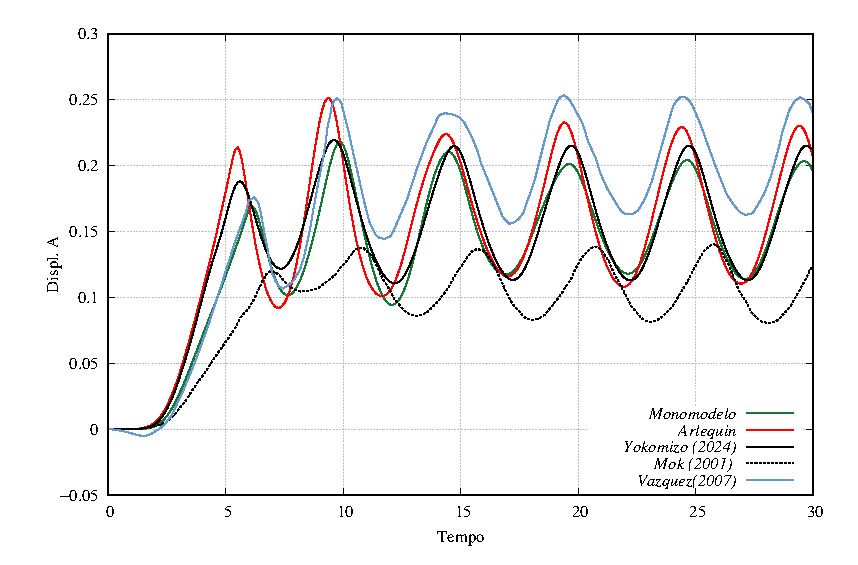
\includegraphics[scale=1.0,trim=0cm 0cm 0cm 0cm, clip=true]{Imagens/Cap7/Cav3dDisplacement.eps}	
	\caption{Cavidade fundo flexível 3D: Deslocamento em A}
	\label{fig:cavidadeFF2d_DeslocamentoemA}
\end{figure}

\textcolor{red}{rever aqui}
Rodar denovo o monomodelo 3d
ALTERAR FIGURA ANTERIOR
ADICIONAR AQUI imagens da velocidade e pressão.
ADICIONAR AQUI imagens do campo de deslocamentos na placa.


\subsection{\textit{Flutter} em painel flexível}

O problema dessa subseção consiste em um painel flexível engastado a um prisma rígido, conforme Fig. \ref{fig:Painel:Geometria}. Devido a complexidade dos fenômenos envolvidos nessa simulação, esse exemplo caracteriza-se por ser um dos mais utilizados na literatura para validação de formulações de IFE. Esse problema foi inicialmente proposto por \citeonline{WallR:1998}, e mais tarde, reformulado por \citeonline{Hubneretal:2004}. Essa segunda versão apresenta a mesma geometria da original, entretanto, possui alteração na velocidade de entrada e nas propriedades elásticas da estrutura. A versão apresentada por \citeonline{Hubneretal:2004}, será utilizada nesse estudo, e distingue-se por ser menos propícia a instabilidades decorrentes de acoplamento fraco. Esse problema apresenta comportamento bidimensional e aqui será simulado através de uma malha 3D utilizando-se uma profundidade de 0,1cm.

\begin{figure}[htb!]
	\centering 
	\includegraphics[scale=0.5,trim=0cm 0cm 0cm 0cm, clip=true]{Imagens/Cap7/prismaGeo.pdf}	
	\caption{Painel Flexível: Geometria}
	\label{fig:Painel:Geometria}
\end{figure}

A velocidade de entrada do escoamento é definida por $u_{\infty} = 31,5 cm/s$ e o fluido possui propriedades físicas do ar: $\viscosity=1,82\times10^{-4} g/(cm.s)$ e $\rho_{f} = 1,18\times10^{-3} g/cm^3 $. Tomando-se por referência o comprimento do prisma obtém-se um número de Reynolds $\Reynolds = 204$. A placa possui espessura de 0,06cm, $\rho_{e} =  2,0 g/cm^3 $, e $E = 2,0\times10^{5} g/(cm.s^2)$. Devido ao comportamento bidimensional do problema adotou-se $\nu=0,0$ para a placa. 

Para a simulação adotou-se para o campo de velocidade inicial $u_{\infty}$. As condições de contorno para o problema são apresentadas na Fig. \ref{fig:Painel:Geometria} (com dimensões em cm). Adicionalmente adotou-se condição de simetria para o fluido na direção $y$, e para estrutura, em $y=0,0$ e $y=0,1$, definiu-se vetor generalizado e os deslocamentos, nesta direção, como nulos.

As simulações foram conduzidas utilizando um Modelo Arlequin (Fig. \ref{fig:painelflex_MalhaArlequin}), onde a malha global foi discretizada com elementos isogeométricos quadráticos, enquanto que para malha local foram utilizados elementos finitos tetraédricos quadráticos. Além disso, um monomodelo foi empregado nas análises, discretizado com elementos finitos tetraédricos quadráticos. Em ambos os modelos, a placa foi representada por elementos finitos triangulares quadráticos, conforme ilustrado na Fig. \ref{fig:painelflex_MalhaPlaca}.

\begin{figure}[htb!]
	\centering
	\subfloat[Malhas do modelo Arlequin \label{fig:painelflex_MalhaArlequin}]{\includegraphics[scale=0.3,trim=0cm 11cm 2cm 0cm, clip=true]{Imagens/Cap7/PrismaPF.pdf}}\\ 
	\subfloat[Malha da placa \label{fig:painelflex_MalhaPlaca}]{\includegraphics[scale=0.3,trim=0cm 18cm 0cm 18cm, clip=true]{Imagens/Cap7/malhaPlacaPrisma.pdf}} 
	\caption{Painel Flexível: Discretização}
\end{figure}

O modelo Arlequin é composto por uma malha global discretizada com 1800 elementos e 5952 pontos de controle. A malha local possui 11061 elementos e 22407 nós. A zona de colagem, com espessura de 0,2cm, de acordo com a Fig. \ref{fig:painelflex_MalhaArlequin} é composta por 2979 elementos e 6503 nós.  O monomodelo foi discretizado com 13315 elementos e 26599 nós. A malha da placa é constituída por 273 nós e 108 elementos. No que diz respeito a integração temporal utilizou-se $\timeStep = 5\times10^{-4}$, e $\specRadius = 0,5$.

\citeonline{Hubneretal:2004} obtém em suas simulações uma frequência de desprendimento de vórtices, considerando a placa como rígida, de $f_f = 3,7Hz$. De acordo com a teoria clássica da dinâmica das estruturas as três primeiras frequências naturais de vibração para essa estrutura de placa são $f_1 = 0,61Hz$, $f_2 = 3,80Hz$ e $f_3 = 10,63Hz$. Dessa forma, espera-se que a frequência de vibração da estrutura para o problema de IFE fique próxima a sua segunda frequência natural.

Na Fig. \ref{fig:Painel:DeslocamentoPONTA} pode-se observar os resultados de deslocamento vertical na ponta da placa (ponto A) obtidos nesse estudo através do modelo Arlequin e do Monomodelo. Conforme pode ser observado os resultados para o monomodelo não chegam até o tempo final estimado para análise, isto se deve em função do colapso que ocorre na malha devido aos grandes deslocamentos. A deformação da malha do monomodelo em um tempo anterior ao colapso pode ser observada na Fig. \ref{fig:Painel:ColapsoMono}. Na Fig. \ref{fig:Painel:DeslocamentoPONTA} também podem ser visualizado a envoltória dos deslocamentos obtidos por \citeonline{Hubneretal:2004}. Nota-se que os resultados desse trabalho vão se aproximando com os da referência a medida que o tempo de análise aumenta. A placa desloca-se de maneira crescente até certo ponto da análise, e a partir de então sua amplitude de vibração se mantém aproximadamente constante.

 
\citeonline{Hubneretal:2004} obteve frequência de vibração um valor de $3,1Hz$ enquanto que nesse trabalho obteve-se o valor de ACRESCENTAR VALOR. Com relação a amplitude máxima obtiveram-se valores de +0,78 e -0,78. ALTERAR.

\textcolor{red}{Alterar fogira abaixo}

\begin{figure}[htb!]
	\centering 
	\includegraphics[scale=1.0,trim=0cm 0cm 0cm 0cm, clip=true]{Imagens/Cap7/deslocamentoPONTAPlaca.eps}	
	\caption{Painel Flexível: Deslocamento em A}
	\label{fig:Painel:DeslocamentoPONTA}
\end{figure}

\begin{figure}[htb!]
	\centering 
	\includegraphics[scale=0.25,trim=0cm 0cm 0cm 0cm, clip=true]{Imagens/Cap7/deformadaMonomodelo.pdf}	
	\caption{Painel Flexível: Colapso malha monomodelo}
	\label{fig:Painel:ColapsoMono}
\end{figure}

Considerando um ciclo de movimento da estrutura $T$ (aproximadamente periódico) apresentam-se os valores de campos de velocidade (Fig. ) e de pressão (Fig) para alguns instantes dentro do ciclo. Na Fig. apresentam-se as deformações da malha para o problema nesses mesmos instantes.

\textcolor{red}{Adicionar Figuras}
	

\end{document}
